
\section{Topics covered}
\begin{itemize}

\item Change management

\item Version management

\item System building

\item Release management

\end{itemize}

\section{Configuration management}
\begin{itemize}

\item Because software changes frequently, systems, can be thought of as a set of versions, each of which has to be maintained and managed.

\item Versions implement proposals for change, corrections of faults, and adaptations for different hardware and operating systems.

\item Configuration management (CM) is concerned with the policies, processes and tools for managing changing software systems. You need CM because it is easy to lose track of what changes and component versions have been incorporated into each system version.

\end{itemize}
\section{CM activities}
\begin{itemize}

\item Change management

   \item Keeping track of requests for changes to the software from customers and developers, working out the costs and impact of changes, and deciding the changes should be implemented.

\item Version management

   \item Keeping track of the multiple versions of system components and ensuring that changes made to components by different developers do not interfere with each other.

\item System building

   \item The process of assembling program components, data and libraries, then compiling these to create an executable system.

\item Release management

   \item Preparing software for external release and keeping track of the system versions that have been released for customer use.
\end{itemize}

\section{Configuration management activities}
\begin{figure}[h!]
    \centering
    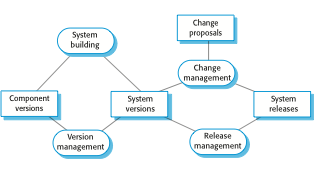
\includegraphics[width = 0.8\textwidth]{./figures/L8_1.png}
    \caption{}
    \label{fig:L8_1}
\end{figure}

\newpage
\section{CM terminology}
\begin{longtable}{|p{2cm}|p{10cm}|}
% \centering
% \begin{tabular}{ |p{2cm}|p{10cm}|  }
\hline
Term & Explanation \\
\hline
\hline
Configuration item or software configuration item (SCI) & Anything associated with a software project (design, code, test data, document, etc.) that has been placed under configuration control. There are often different versions of a configuration item. Configuration items have a unique name.\\
\hline
Configuration control & The process of ensuring that versions of systems and components are recorded and maintained so that changes are managed and all versions of components are identified and stored for the lifetime of the system.\\
\hline
Version & An instance of a configuration item that differs, in some way, from other instances of that item. Versions always have a unique identifier, which is often composed of the configuration item name plus a version number.\\
\hline
Baseline & A baseline is a collection of component versions that make up a system. Baselines are controlled, which means that the versions of the components making up the system cannot be changed. This means that it should always be possible to recreate a baseline from its constituent components.\\
\hline
Codeline & A codeline is a set of versions of a software component and other configuration items on which that component depends.\\
\hline
Mainline & A sequence of baselines representing different versions of a system.\\
\hline
Release & A version of a system that has been released to customers (or other users in an organization) for use.\\
\hline
Workspace & A private work area where software can be modified without affecting other developers who may be using or modifying that software.\\
\hline
Branching & The creation of a new codeline from a version in an existing codeline. The new codeline and the existing codeline may then develop independently.\\
\hline
Merging & The creation of a new version of a software component by merging separate versions in different codelines. These codelines may have been created by a previous branch of one of the codelines involved.\\
\hline
System building & The creation of an executable system version by compiling and linking the appropriate versions of the components and libraries making up the system.\\
\hline
% \end{tabular}
\caption{}
\label{table:T6_2}
\end{longtable}


% \newpage
\section{Change management}
\begin{itemize}

\item Organizational needs and requirements change during the lifetime of a system, bugs have to be repaired and systems have to adapt to changes in their environment.

\item Change management is intended to ensure that system evolution is a managed process and that priority is given to the most urgent and cost-effective changes.

\item The change management process is concerned with analyzing the costs and benefits of proposed changes, approving those changes that are worthwhile and tracking which components in the system have been changed.

\end{itemize}
\section{The change management process}
\begin{figure}[h!]
    \centering
    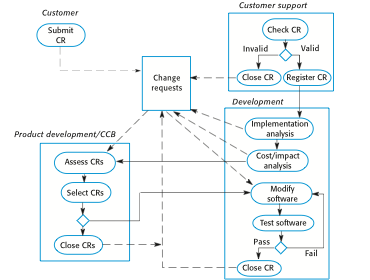
\includegraphics[width = 0.8\textwidth]{./figures/L8_2.png}
    \caption{}
    \label{fig:L8_2}
\end{figure}


\section{A partially completed change request form (a)}


Change Request Form
\begin{description}
  \item[Project:] SICSA/AppProcessing
  \item[Number:] 23/02
  \item[Change requester:] I. Sommerville
  \item[Date:] 20/01/09
  \item[Requested change:] The status of applicants (rejected, accepted, etc.) should be shown visually in the displayed list of applicants.
  \item[Change analyzer:] R. Looek
  \item[Analysis date:] 25/01/09
  \item[Components affected:] ApplicantListDisplay, StatusUpdater
  \item[Associated components:] StudentDatabase
\end{description}



\section{A partially completed change request form (b)}

Change Request Form
\begin{description}
  \item[Change assessment:]Relatively simple to implement by changing the display color according to status. A table must be added to relate status to colors. No changes to associated components are required.
  \item[Change priority:]Medium
  \item[Change implementation:]
  \item[Estimated effort:]2 hours
  \item[Date to SGA app. team:] 28/01/09
  \item[CCB decision date:] 30/01/09
  \item[Decision:] Accept change. Change to be implemented in Release 1.2

  \item[Change implementor:]
  \item[Date submitted to QA:]
  \item[Date submitted to CM:]
  \item[Comments:]
  \item[Date of change: QA decision:]

\end{description}







\section{Factors in change analysis}
\begin{itemize}

\item The consequences of not making the change

\item The benefits of the change

\item The number of users affected by the change

\item The costs of making the change

\item The product release cycle

\end{itemize}
\section{Change management and agile methods}
\begin{itemize}
\item In some agile methods, customers are directly involved in change management.

\item The propose a change to the requirements and work with the team to assess its impact and decide whether the change should take priority over the features planned for the next increment of the system.

\item Changes to improve the software improvement are decided by the programmers working on the system.

\item Refactoring, where the software is continually improved, is not seen as an overhead but as a necessary part of the development process.

\end{itemize}
\section{Derivation history}


SICSA project (XEP 6087)
\newline
APP-SYSTEM\/AUTH\/RBAC\/USER\_ROLE
\newline
Object: currentRole
\newline
Author: R. Looek
\newline
Creation date: 13/11/2009
\newline
© St Andrews University 2009
\newline
Modification history
\newline
Version Modifier Date	Change	Reason

\newpage
\begin{table}[h!]
\centering
\begin{tabular}{ |p{4cm}|p{4cm}|  }
\hline
1.0	J. Jones & 1.1	R. Looek\\
\hline
11/11/2009 & 13/11/2009\\
\hline
Add header & New field\\
\hline
Submitted to CM & Change req. R07/02\\
\hline
\end{tabular}

\label{table:T6_3}
\end{table}

\section{Version management}
\begin{itemize}
\item Version management (VM) is the process of keeping track of different versions of software components or configuration items and the systems in which these components are used.

\item It also involves ensuring that changes made by different developers to these versions do not interfere with each other.

\item Therefore version management can be thought of as the process of managing codelines and baselines.
Codelines and baselines
\item A codelineis a sequence of versions of source code with later versions in the sequence derived from earlier versions.

\item Codelinesnormally apply to components of systems so that there are different versions of each component.

\item A baseline is a definition of a specific system.

\item The baseline therefore specifies the component versions that are included in the system plus a specification of the libraries used, configuration files, etc.


\end{itemize}



\section{Baselines}
\begin{itemize}
\item Baselines may be specified using a configuration language, which allows you to define what components are included in a version of a particular system.

\item Baselines are important because you often have to recreate a specific version of a complete system.

   \item For example, a product line may be instantiated so that there are individual system versions for different customers. You may have to recreate the version delivered to a specific customer if, for example, that customer reports bugs in their system that have to be repaired.
\end{itemize}

\section{Codelinesand baselines}
\begin{figure}[h!]
    \centering
    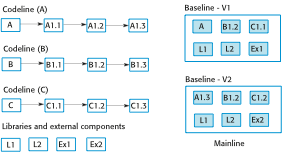
\includegraphics[width = 0.8\textwidth]{./figures/L8_3.png}
    \caption{}
    \label{fig:L8_3}
\end{figure}
\section{Version management systems}
\begin{itemize}

\item Version and release identification

   \item Managed versions are assigned identifiers when they are submitted to the system.

\item Storage management

   \item To reduce the storage space required by multiple versions of components that differ only slightly, version management systems usually provide storage management facilities.

\item Change history recording

   \item All of the changes made to the code of a system or component are recorded and listed.

\end{itemize}
\section{Version management systems}
\begin{itemize}

\item Independent development

   \item The version management system keeps track of components that have been checked out for editing and ensures that changes made to a component by different developers do not interfere.

\item Project support

   \item A version management system may support the development of several projects, which share components.


\end{itemize}
\section{Storage management using deltas}
\begin{figure}[h!]
    \centering
    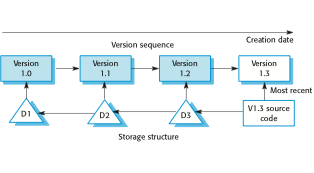
\includegraphics[width = 0.8\textwidth]{./figures/L8_4.png}
    \caption{}
    \label{fig:L8_4}
\end{figure}

\section{Check-in and check-out from a version repository}
\begin{figure}[h!]
    \centering
    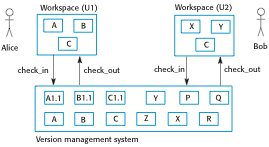
\includegraphics[width = 0.8\textwidth]{./figures/L8_5.png}
    \caption{}
    \label{fig:L8_5}
\end{figure}


\section{Codeline branches}
\begin{itemize}

\item Rather than a linear sequence of versions that reflect changes to the component over time, there may be several independent sequences.

   \item This is normal in system development, where different developers work independently on different versions of the source code and so change it in different ways.

\item At some stage, it may be necessary to merge codeline branches to create a new version of a component that includes all changes that have been made.

   \item If the changes made involve different parts of the code, the component versions may be merged automatically by combining the deltas that apply to the code.

\end{itemize}
\section{Branching and merging}
\begin{figure}[h!]
    \centering
    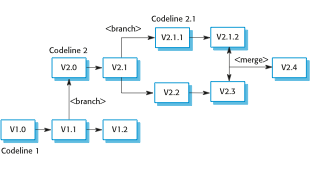
\includegraphics[width = 0.8\textwidth]{./figures/L8_6.png}
    \caption{}
    \label{fig:L8_6}
\end{figure}




\section{Key points}
\begin{itemize}

\item Configuration management is the management of an evolving software system. When maintaining a system, a CM team is put in place to ensure that changes are incorporated into the system in a controlled way and that records are maintained with details of the changes that have been implemented.

\item The main configuration management processes are change management, version management, system building and release management.

\item Change management involves assessing proposals for changes from system customers and other stakeholders and deciding if it is cost-effective to implement these in a new version of a system.

\item Version management involves keeping track of the different versions of software components as changes are made to them.
\end{itemize}
\section{System building}
\begin{itemize}

\item System building is the process of creating a complete, executable system by compiling and linking the system components, external libraries, configuration files, etc.

\item System building tools and version management tools must communicate as the build process involves checking out component versions from the repository managed by the version management system.

\item The configuration description used to identify a baseline is also used by the system building tool.


\end{itemize}
\section{B platforms}
\begin{itemize}
\item The development system, which includes development tools such as compilers, source code editors, etc.

   \item Developers check out code from the version management system into a private workspace before making changes to the system.

\item The build server, which is used to build definitive, executable versions of the system.

   \item Developers check-in code to the version management system before it is built. The system build may rely on external libraries that are not included in the version management system.

\item The target environment, which is the platform on which the system executes.
\newpage
\section{Development, build, and target platforms}
\begin{figure}[h!]
    \centering
    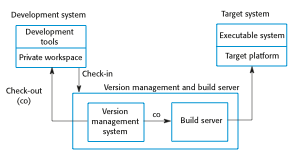
\includegraphics[width = 0.8\textwidth]{./figures/L8_7.png}
    \caption{}
    \label{fig:L8_7}
\end{figure}



\end{itemize}
\section{System building}

\begin{figure}[h!]
    \centering
    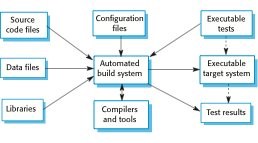
\includegraphics[width = 0.8\textwidth]{./figures/L8_8.png}
    \caption{}
    \label{fig:L8_8}
\end{figure}



\section{Build system functionality}
\begin{itemize}

\item Build script generation

\item Version management system integration

\item Minimal re-compilation

\item Executable system creation

\item Test automation

\item Reporting

\item Documentation generation

\end{itemize}
\section{Minimizing recompilation}
\begin{itemize}
\item Tools to support system building are usually designed to minimize the amount of compilation that is required.

\item They do this by checking if a compiled version of a component is available. If so, there is no need to recompile that component.

\item A unique signature identifies each source and object code version and is changed when the source code is edited.

\item By comparing the signatures on the source and object code files, it is possible to decide if the source code was used to generate the object code component.
\end{itemize}
\section{File identification}
\begin{itemize}
\item Modification timestamps

   \item The signature on the source code file is the time and date when that file was modified. If the source code file of a component has been modified after the related object code file, then the system assumes that recompilation to create a new object code file is necessary.

\item Source code checksums

   \item The signature on the source code file is a checksum calculated from data in the file. A checksum function calculates a unique number using the source text as input. If you change the source code (even by 1 character), this will generate a different checksum. You can therefore be confident that source code files with different checksums are actually different.

\end{itemize}
\section{Timestamps vs checksums}
\begin{itemize}

\item Timestamps

   \item Because source and object files are linked by name rather than an explicit source file signature, it is not usually possible to build different versions of a source code component into the same directory at the same time, as these would generate object files with the same name.

\item Checksums

   \item When you recompile a component, it does not overwrite the object code, as would normally be the case when the timestamp is used. Rather, it generates a new object code file and tags it with the source code signature. Parallel compilation is possible and different versions of a component may be compiled at the same time.
\end{itemize}
\section{Agile building}
\begin{itemize}

\item Check out the mainline system from the version management system into the developer’s private workspace.

\item Build the system and run automated tests to ensure that the built system passes all tests. If not, the build is broken and you should inform whoever checked in the last baseline system. They are responsible for repairing the problem.

\item Make the changes to the system components.

\item Build the system in the private workspace and rerun system tests. If the tests fail, continue editing.


\end{itemize}
\section{Agile building}
\begin{itemize}

\item Once the system has passed its tests, check it into the build system but do not commit it as a new system baseline.

\item Build the system on the build server and run the tests. You need to do this in case others have modified components since you checked out the system. If this is the case, check out the components that have failed and edit these so that tests pass on your private workspace.

\item If the system passes its tests on the build system, then commit the changes you have made as a new baseline in the system mainline.
\end{itemize}

\newpage
\section{Continuous integration}
\begin{figure}[h!]
    \centering
    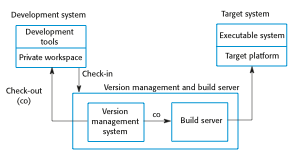
\includegraphics[width = 0.8\textwidth]{./figures/L8_7.png}
    \caption{}
    \label{fig:L8_9}
\end{figure}


\section{Daily building}
\begin{itemize}

\item The development organization sets a delivery time (say 2 p.m.) for system components.

   \item If developers have new versions of the components that they are writing, they must deliver them by that time.
   \item A new version of the system is built from these components by compiling and linking them to form a complete system.
   \item This system is then delivered to the testing team, which carries out a set of predefined system tests
   \item Faults that are discovered during system testing are documented and returned to the system developers. They repair these faults in a subsequent version of the component.

\end{itemize}
\section{Release management}
\begin{itemize}

\item A system release is a version of a software system that is distributed to customers.

\item For mass market software, it is usually possible to identify two types of release: major releases which deliver significant new functionality, and minor releases, which repair bugs and fix customer problems that have been reported.

\item For custom software or software product lines, releases of the system may have to be produced for each customer and individual customers may be running several different releases of the system at the same time.
\end{itemize}
\section{Release tracking}
\begin{itemize}

\item In the event of a problem, it may be necessary to reproduce exactly the software that has been delivered to a particular customer.

\item When a system release is produced, it must be documented to ensure that it can be re-created exactly in the future.

\item This is particularly important for customized, long-lifetime embedded systems, such as those that control complex machines.

   \item Customers may use a single release of these systems for many years and may require specific changes to a particular software system long after its original release date.
\end{itemize}
\section{Release reproduction}
\begin{itemize}
\item To document a release, you have to record the specific versions of the source code components that were used to create the executable code.

\item You must keep copies of the source code files, corresponding executables and all data and configuration files.

\item You should also record the versions of the operating system, libraries, compilers and other tools used to build the software.

\end{itemize}
\section{Release planning}
\begin{itemize}

\item As well as the technical work involved in creating a release distribution, advertising and publicity material have to be prepared and marketing strategies put in place to convince customers to buy the new release of the system.

\item Release timing

   \item If releases are too frequent or require hardware upgrades, customers may not move to the new release, especially if they have to pay for it.
   \item If system releases are too infrequent, market share may be lost as customers move to alternative systems.

\end{itemize}
\section{Release components}
\begin{itemize}

\item As well as the the executable code of the system, a release may also include:

   \item configuration files defining how the release should be configured for particular installations;
   \item data files, such as files of error messages, that are needed for successful system operation;
   \item an installation program that is used to help install the system on target hardware;
   \item electronic and paper documentation describing the system;

   \item packaging and associated publicitythat have been designed for that release.

\end{itemize}
\section{Factors influencing system release planning}
\begin{table}[h!]
\centering
\begin{tabular}{ |p{3cm}|p{8cm}|  }
\hline
Factor & Description \\
\hline
\hline
Technical quality of the system & If serious system faults are reported which affect the way in which many customers use the system, it may be necessary to issue a fault repair release. Minor system faults may be repaired by issuing patches (usually distributed over the Internet) that can be applied to the current release of the system.\\
\hline
Platform changes & You may have to create a new release of a software application when a new version of the operating system platform is released.\\
\hline
Lehman’s fifth law (see Chapter 9) & This ‘law’ suggests that if you add a lot of new functionality to a system; you will also introduce bugs that will limit the amount of functionality that may be included in the next release. Therefore, a system release with significant new functionality may have to be followed by a release that focuses on repairing problems and improving performance.\\
\hline
Competition & For mass-market software, a new system release may be necessary because a competing product has introduced new features and market share may be lost if these are not provided to existing customers.\\
\hline
Marketing requirements & The marketing department of an organization may have made a commitment for releases to be available at a particular date.\\
\hline
Customer change proposals & For custom systems, customers may have made and paid for a specific set of system change proposals, and they expect a system release as soon as these have been implemented.\\
\hline
\end{tabular}

\label{table:T6_2}
\end{table}

\section{Key points}
\begin{itemize}
\item System building is the process of assembling system components into an executable program to run on a target computer system.

\item Software should be frequently rebuilt and tested immediately after a new version has been built. This makes it easier to detect bugs and problems that have been introduced since the last build.

\item System releases include executable code, data files, configuration files and documentation. Release management involves making decisions on system release dates, preparing all information for distribution and documenting each system release.
\end{itemize}
